% $Id: template.tex 11 2007-04-03 22:25:53Z jpeltier $

\documentclass{vgtc}                          % final (conference style)
%\documentclass[review]{vgtc}                 % review
%\documentclass[widereview]{vgtc}             % wide-spaced review
%\documentclass[preprint]{vgtc}               % preprint
%\documentclass[electronic]{vgtc}             % electronic version

%% Uncomment one of the lines above depending on where your paper is
%% in the conference process. ``review'' and ``widereview'' are for review
%% submission, ``preprint'' is for pre-publication, and the final version
%% doesn't use a specific qualifier. Further, ``electronic'' includes
%% hyperreferences for more convenient online viewing.

%% Please use one of the ``review'' options in combination with the
%% assigned online id (see below) ONLY if your paper uses a double blind
%% review process. Some conferences, like IEEE Vis and InfoVis, have NOT
%% in the past.

%% Figures should be in CMYK or Grey scale format, otherwise, colour 
%% shifting may occur during the printing process.

%% These few lines make a distinction between latex and pdflatex calls and they
%% bring in essential packages for graphics and font handling.
%% Note that due to the \DeclareGraphicsExtensions{} call it is no longer necessary
%% to provide the the path and extension of a graphics file:
%% \includegraphics{diamondrule} is completely sufficient.
%%
\ifpdf%                                % if we use pdflatex
  \pdfoutput=1\relax                   % create PDFs from pdfLaTeX
  \pdfcompresslevel=9                  % PDF Compression
  \pdfoptionpdfminorversion=7          % create PDF 1.7
  \ExecuteOptions{pdftex}
  \usepackage{graphicx}                % allow us to embed graphics files
  \DeclareGraphicsExtensions{.pdf,.png,.jpg,.jpeg} % for pdflatex we expect .pdf, .png, or .jpg files
\else%                                 % else we use pure latex
  \ExecuteOptions{dvips}
  \usepackage{graphicx}                % allow us to embed graphics files
  \DeclareGraphicsExtensions{.eps}     % for pure latex we expect eps files
\fi%

%% it is recomended to use ``\autoref{sec:bla}'' instead of ``Fig.~\ref{sec:bla}''
\graphicspath{{figures/}{pictures/}{images/}{./}} % where to search for the images

\usepackage{microtype}                 % use micro-typography (slightly more compact, better to read)
\PassOptionsToPackage{warn}{textcomp}  % to address font issues with \textrightarrow
\usepackage{textcomp}                  % use better special symbols
\usepackage{mathptmx}                  % use matching math font
\usepackage{times}                     % we use Times as the main font
\renewcommand*\ttdefault{txtt}         % a nicer typewriter font
\usepackage{cite}                      % needed to automatically sort the references
\usepackage{tabu}                      % only used for the table example
\usepackage{booktabs}                  % only used for the table example
%% We encourage the use of mathptmx for consistent usage of times font
%% throughout the proceedings. However, if you encounter conflicts
%% with other math-related packages, you may want to disable it.


%% If you are submitting a paper to a conference for review with a double
%% blind reviewing process, please replace the value ``0'' below with your
%% OnlineID. Otherwise, you may safely leave it at ``0''.
\onlineid{0}

%% declare the category of your paper, only shown in review mode
\vgtccategory{Research}

%% allow for this line if you want the electronic option to work properly
\vgtcinsertpkg

%% In preprint mode you may define your own headline.
%\preprinttext{To appear in an IEEE VGTC sponsored conference.}

%% Paper title.

\title{Reconstructing the MRI Aesthetic}

%% This is how authors are specified in the conference style

%% Author and Affiliation (single author).
%%\author{Roy G. Biv\thanks{e-mail: roy.g.biv@aol.com}}
%%\affiliation{\scriptsize Allied Widgets Research}

%% Author and Affiliation (multiple authors with single affiliations).
%%\author{Roy G. Biv\thanks{e-mail: roy.g.biv@aol.com} %
%%\and Ed Grimley\thanks{e-mail:ed.grimley@aol.com} %
%%\and Martha Stewart\thanks{e-mail:martha.stewart@marthastewart.com}}
%%\affiliation{\scriptsize Martha Stewart Enterprises \\ Microsoft Research}

%% Author and Affiliation (multiple authors with multiple affiliations)
\author{Michael Page\thanks{e-mail: mpage@faculty.ocadu.ca}\\ %
        \scriptsize OCAD University %
\and Marcus Gordon\thanks{e-mail: mgordon@faculty.ocadu.ca}\\ %
        \scriptsize OCAD University %
\and Mario Garingo\thanks{e-mail: mgaringo@faculty.ocadu.ca}\\ %
        \scriptsize OCAD University %
\and Adriana Menghi\thanks{e-mail: adriana.menghi@mail.utoronto.ca}\\ %
        \scriptsize OCAD University %
\and Jawa El Khash\thanks{e-mail: jelkhash@faculty.ocadu.ca}\\ %
        \scriptsize OCAD University %
}

%% A teaser figure can be included as follows, but is not recommended since
%% the space is now taken up by a full width abstract.
%\teaser{
%  \includegraphics[width=1.5in]{sample.eps}
%  \caption{Lookit! Lookit!}
%}

%% Abstract section.
\abstract{In this work we present a visualization pipeline to express a series of magnetic resonance imaging (MRI) volume data, as a full coloured hologram.  We believe our pipeline can highlight salient structure information which reside within the data without extensive processing of the raw MRI, by utilizing its spatial and temporal characteristics.  Our unique approach on MRI visualization highlight the importance of using the right colormap and the untapped use of holograms in the medical field to give depth information.  We employ artist-driven colour techniques which make use of luminance and saturation rather than the current standard of contrast of hues. Our poster will provide a brief overview of the current spatial displays in medical imaging application and describe both the current process of processing an MRI dataset, through model construction, computer graphic rendering, and hologram encoding to our proposed pipeline of: MRI dataset, colour mapping, hologram encoding.  We show the results of our pipeline and highlight various structures within the data without the use of sophisticated segmentation techniques.
} % end of abstract


\CCScatlist{
  \CCScatTwelve{Human-centered computing}{Visu\-al\-iza\-tion}{Visu\-al\-iza\-tion techniques}{Treemaps};
  \CCScatTwelve{Human-centered computing}{Visu\-al\-iza\-tion}{Visualization design and evaluation methods}{}
}

%%%%%%%%%%%%%%%%%%%%%%%%%%%%%%%%%%%%%%%%%%%%%%%%%%%%%%%%%%%%%%%%
%%%%%%%%%%%%%%%%%%%%%% START OF THE PAPER %%%%%%%%%%%%%%%%%%%%%%
%%%%%%%%%%%%%%%%%%%%%%%%%%%%%%%%%%%%%%%%%%%%%%%%%%%%%%%%%%%%%%%%%

\begin{document}


\firstsection{Introduction}
\maketitle
In medicine, doctors rely on visualization tools to display tumor or any other lesions, in a clear manner such that the spatial relationship to anatomical structures of the brain are perceived.  Typically, they use magnetic resonance images (MRI) to obtain volumetric data and display them onto a monitor.  They manipulated the 3D data, inherent to MRI, as 2D data through a monitor.  These visualization tools often show various angles of the data so that the physician can infer the relative position, orientation, shape and relevant anatomical cues to disambiguate the spatial relationship between the tumor and the rest of the brain structure.\\

We hypothesize that viewing 3D structured data is best viewed using true 3D displays such as holograms. We believe that it can be more effective in representing the tumors shape and position especially in situations when the shape is abnormal and the tissue is statistically similar to its surrounding.  Furthermore, holograms has an additional advantage to other 3D displays in that  no special viewing aids are needed such as special glasses or a head worn display such as a VR headset.  \\

In addition because holograms are in colour we can utilize different color mapping technique to highlight various regions in the MRI without manipulating the data, which is a necessity in the medical field.  Furthermore, in the past depth was used as a colour parameter but using holograms depth is inherent so we can use the raw data as parameters for colour instead. In the literature it has been established that with the appropriate colour mapping techniques colormaps play an important role in visualization because they are able to improve the efficiency and effectiveness of data perception which in turn allow more insights into the data.\\  

The main focus and contribution of this poster is to highlight the importance of colour as well as the visualization medium to optimally view medical volumetric data such as MRIs, and provide an alternative visualization pipeline to viewing them.



\section{Theory}
\begin{figure}[tb]
 \centering % avoid the use of \begin{center}...\end{center} and use \centering instead (more compact)
 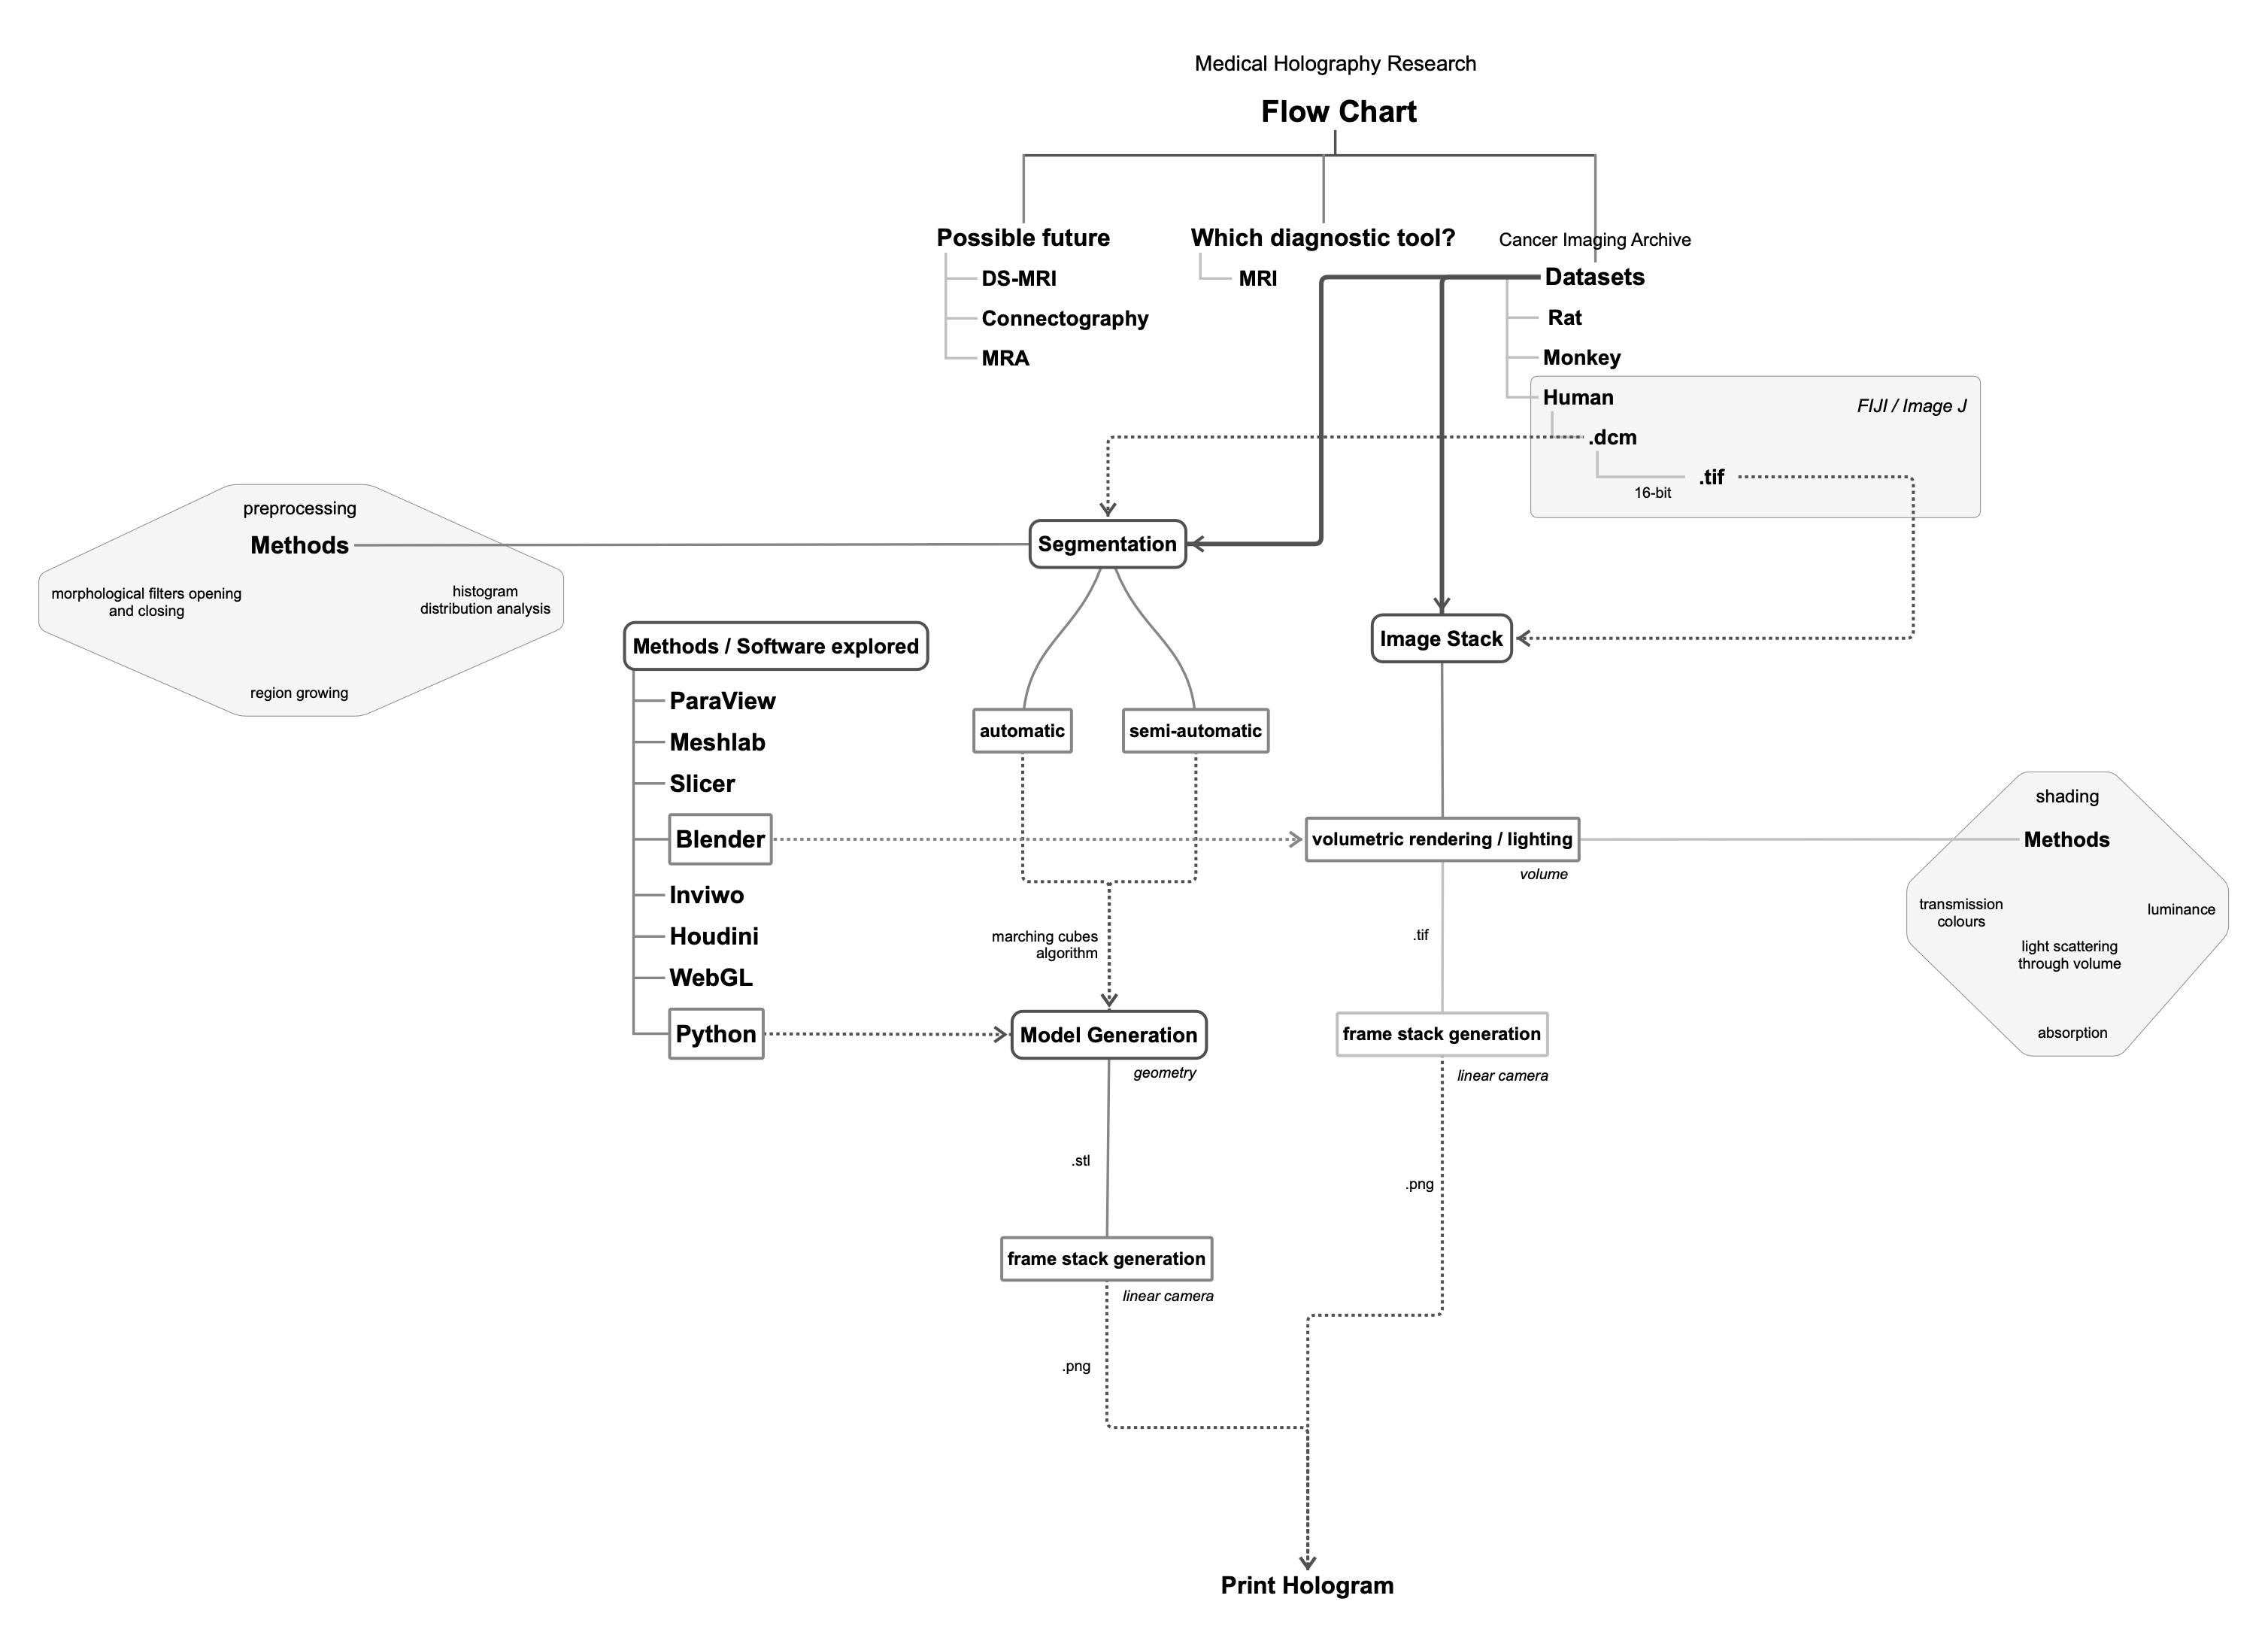
\includegraphics[width=\columnwidth]{pictures/detailedFlowChart.png}
 \caption{The left path of the above flowchart diagram shows the current methods in generating medical holographic prints. The right path of the above flowchart diagram shows our proposed method.} 
 \label{fig:flowChart}
\end{figure}


\subsection{Colour Mapping, an Artist-Driven Colour Method Approach}
In the literature as well as in most scientific visualization programs, colour has been proven to be an effective tool.  However, no single color-map is optimized for all science domains.  Current default colour schemes such as the rainbow, jet, gray-scale and cool to warm often obscure data and fail to solve the occlusion relationships in volumetric rendering of data.  There have been work in this field to combat this issue and user-study-based, rule-based and data-driven methods have been explored.  Whoever we believe that the work done by [Samel] is the most effective method in solving this occlusion problem.  We extend their work into the 3D medical field by applying two principle from artistic colour theory: maximizing values contrast and avoiding simultaneity of colour.\\

Humans ability to focus attention and discriminate detail is governed by the type and degree of contrast and not by specific hues.  In our case-study of using a human brain and tumor, it is essential for the tumor to be apparent and salient in the scene.  One major pitfall of the current colour schemes is the visual vibration caused by the abutting saturated hues of the colourmaps.  As a result our mapping system will focus more on the allocation of contrast, specifically luminance and saturation. Hence we use the following colour schemes:\\

\begin{figure}[h]
 \centering % avoid the use of \begin{center}...\end{center} and use \centering instead (more compact)
 
\includegraphics[width=\columnwidth]{pictures/orange-5.png}
 \caption{Linear Colormap from ColorMoves.}
 \label{fig:orange5}
\end{figure}

\begin{figure}[h]
 \centering % avoid the use of \begin{center}...\end{center} and use \centering instead (more compact)
 
\includegraphics[width=\columnwidth]{pictures/divergent-1.png}
 \caption{Divergent Colormap from ColorMoves.}
 \label{fig:divergent1}
\end{figure}

\begin{figure}[h]
 \centering % avoid the use of \begin{center}...\end{center} and use \centering instead (more compact)
 
\includegraphics[width=\columnwidth]{pictures/altstruct-1.png}
 \caption{Structured Colormap from ColorMoves.}
 \label{fig:struct1}
\end{figure}

\subsection{Volumetric Rendering}
The current approach that our group has been using to generate medical holograms is first constructing a model using segmentation. For this we employ an intuitive approach of pixel classification using multi-thresholding  techniques in combination with region growing approaches.  Following this step we perform computer graphic rendering, and hologram encoding.  There are three main issues with pipeline.  The first being a non-automatic method which involves human intervention, second is that it is computationally expensive, and the third is that it generates occlusion between the geometry in the scene.\\

Occlusion is an important and powerful cue to scene layout, and based on psychology studies it usually caries the precept even in the presence of conflicting information.  Analogous to colour, the rendering approach should also report the occlusion relationship between objects within the scene. In this diagnostic application it is important not to hide information of potential interest.  As a result, the semi-transparent and non-occluding nature of volumetric rendering maybe appropriate for some medical diagnostic applications.\\

Volume rendering (technically known as direct volume rendering) in the field of computer graphics is considered to be a form of 3D scalar field.  Its a 3D random density plot composed of spheres that pertain to a particular colour, that essential emit light without any reflectance.  Our approach uses a texture-based volumetric rendering to generate the views of the medical images, capable of being handled by powerful graphics cards yielding quick results and real-time interaction.\\

Combining this approach with the results from luminance distribution tests with colormaps, we create a multivariate workflow of exploring volume data and representing high quality views needed for analysis.  3D volume segmentation techniques are further explored applying luminance distribution in other ways including using a dual colormap strategy in our volume rendering for greater lighting control, and shifting the order of image processing tasks such as applying colourmaps to independent slices versus the direct volume.\\

\subsection{Holograms}
Although the geometry is three dimensional, the holographic printer works by virtually photographing two dimensional image sequences.  These sequences (or frames) are put together as stack, and fed to the  digital holographic printer.  Using a spatial light modulator, the printer invokes a pixel swapping algorithm that connects the various points in 2D space, adding relational z-depth cue information thus forming a three dimensional recording.\\

This process of creating an image stack is necessary to feed information to the printer, and is crucial in generating the overall scene design of the hologram viewed by the observer. As a result, we explore two image processing avenues using a set of 8-bit color images and a set of higher color depth images to compare aesthetic differences. 32-bit HDR images are of interest to investigate further in formats such as OpenEXR \cite{kainz2009technical}. However, due to the nature of creating an HDR image requires either bracketed capture from the imaging device, or the making of 32-bit images directly from the source, we opt for investigating this scenario in the next stage of the research. Additional challenges surfaced when researching the use of OpenEXR and the accessible toolbox of choice of software including Photoshop CC 2019, which at the time writing this, only supported exporting 16-bit OpenEXR files (half float).  ImageMagick, another tool of choice, a command line interface (CLI), also limited use of OpenEXR to 16-bit.\\

In addition to working with HDR images, working with linear colour space is to be considered throughout the pipeline until applying gamma correction for display purposes.  All monochromatic wavelengths are mapped to what is known as the ``spectral locus" of the CIE xy chromaticity diagram \cite{mansencal_thomas_2018_2647615} \cite{reinhard2010high}, familiar territory for holographers when working with colour, lasers, and optics.  Consideration will be given to testing the use of linear colour editing versus the common sRBG colour mode used traditionally with our partners holographic printer.  We believe the digital ``hard copy" nature of our hologram will benefit from looking beyond the sRGB color space.\\

Embedding an understanding of both linear space and gamma space into our workflow, could significantly change the very aesthetic of the images when viewed with color gamuts of digital displays, as such, should have an impact on the experience on the produced digital hologram.  One way to test these differences in our proposed pipeline is to test the making our image stack by incorporating the above stated factors in our production.

\section{Results}
\subsection{Geometry vs Volume}

\subsubsection{Geometry and Image Segmentation}
\subsubsubsection{\textbf{Segmentation}}
In our data set there were 181 slices each containing an image with the dimensions 256x256.  For each slice the segmentation described in the segmentation section of the report was performed to identify each of the known tissues within our dataset.  Figure \ref{fig:resultsHistogram} shows an example the histogram distribution along with their corresponding MRI. Note the distinct peaks of the histogram which corresponds the the distinct known tissues of the brain.\\ 

\begin{figure}[h]
  \centering
  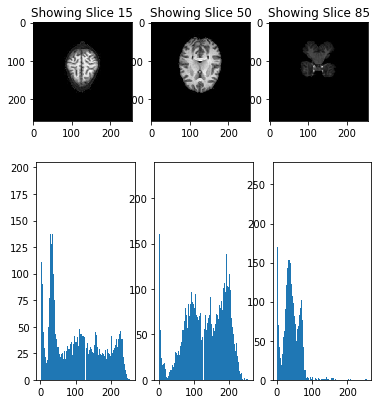
\includegraphics[width=\linewidth]{pictures/resultsHistogram.png}
  \caption{Brain slices of MRI with their corresponding histogram distribution.}
  \label{fig:resultsHistogram}
\end{figure}

Results of the manual seed region growing techniques and morphological filters can be seen in figure \ref{fig:resultsSegmentation}.

\begin{figure}[h]
  \centering
  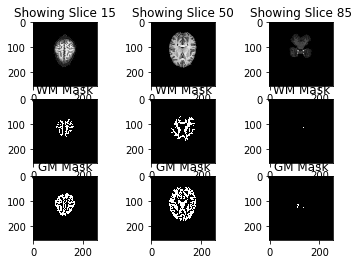
\includegraphics[width=\linewidth]{pictures/resultsSegmentation.png}
  \caption{\textbf{Top Row:} Original MRI. \textbf{Middle Row:}White matter mask. \textbf{Bottom Row:}Gray matter mask.}
  \label{fig:resultsSegmentation}
\end{figure}

We applied this technique not only for the regular brain but also for a brain which contains a tumor.  The following set of figures shows examples slices as well as their resultant class labels and individual mask layers.\\

\begin{figure}[h]
  \centering
  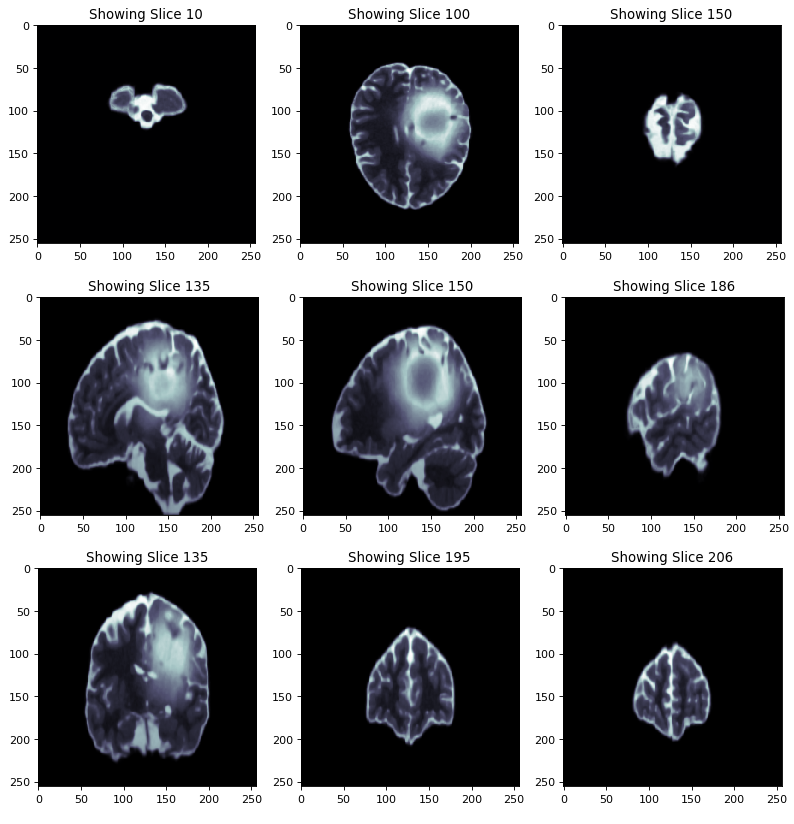
\includegraphics[width=\linewidth]{pictures/originalMRI.png}
  \caption{Original MRI slices in different views.  From top to bottom they are sliced in the axial, sagittal and coronal planes.}
  \label{fig:originalMRI}
\end{figure}

\begin{figure}[h]
  \centering
  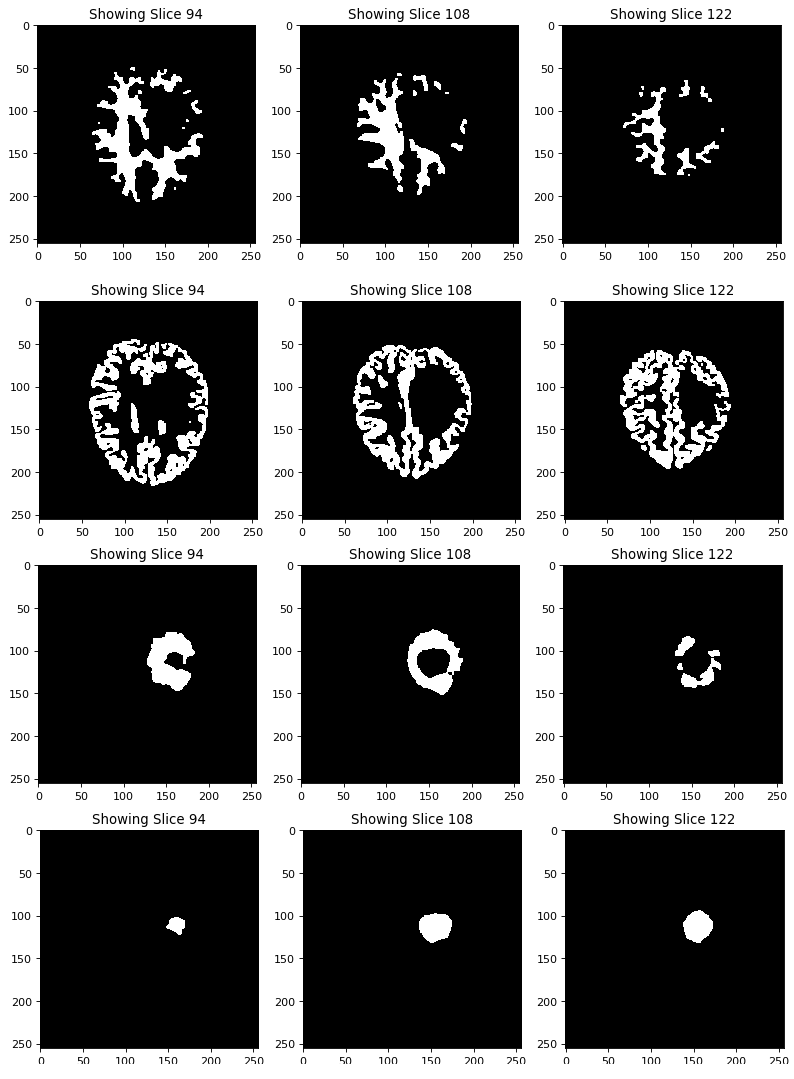
\includegraphics[width=\linewidth]{pictures/resultantMasks.png}
  \caption{Generated masks for each of the known tissue classes in our dataset.  From top to bottom they are: gray matter, white matter, abnormal tissue, and tumor.}
  \label{fig:resultantMasks}
\end{figure}

Even though we applied morphological filters we can still see some noise within the images, specifically the speckle effects in the gray matter and some holes in the white matter masks.\\  

\begin{figure}[h]
  \centering
  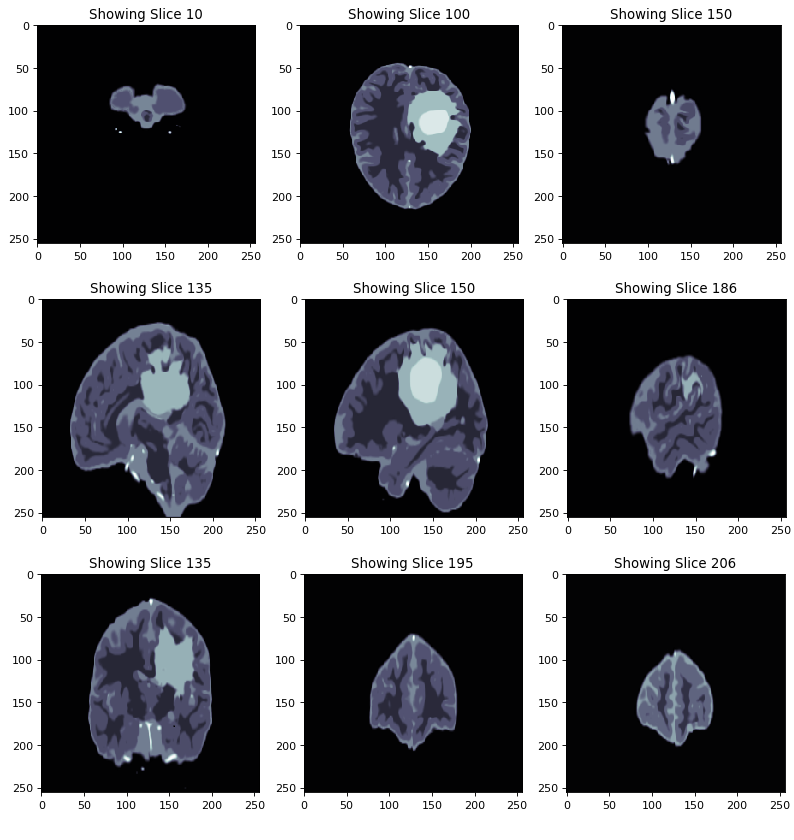
\includegraphics[width=\linewidth]{pictures/labeledMasks.png}
  \caption{Various slices and views of each of the coloured masks as found in the histogram.}
  \label{fig:labeledMasks}
\end{figure}

Each unique colour corresponds to a unique known tissue type.  By looking at various views you can get a picture as to where the tumor maybe located.  To create contrast between each distinct region we proposed the following colouring scheme.

\begin{figure}[h]
  \centering
  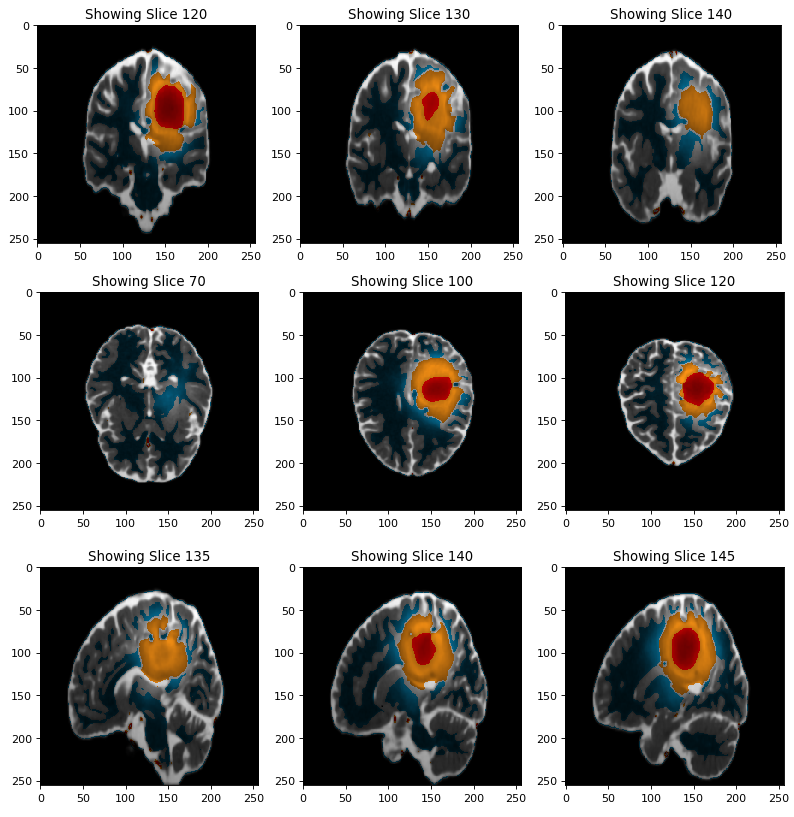
\includegraphics[width=\linewidth]{pictures/colourCodedRegions.png}
  \caption{Colour coded regions of the brain}
  \label{fig:colourCodedRegions}
\end{figure}

\begin{table}[h]
\centering
\begin{tabular}{|r|l|l|l|}
\hline
Tissue & R & \multicolumn{1}{c|}{G} & B \\ \hline
White & 7 & \multicolumn{1}{c|}{150} & 204 \\ \hline
Gray & 204 & 204 & 204 \\ \hline
Abnormal Tissue & 203 & 119 & 17 \\ \hline
Tumor & 203 & 2 & 2 \\ \hline
\end{tabular}
\caption{RGB values of each of the tissue types.}
\label{table:RGBValues}
\end{table}

Notice that for each of the tissue types they can be clearly distinguish from each other. 

\subsubsubsection{\textbf{Geometry Generation}}
From a far it may seem that the models are what we expect but looking at the smaller object such as the tumor and the abnormal tissue it is clear that the resolution of the models are directly correlated with the number of slices within the DICOM file.  The marching cube algorithm generates these step wise artifacts which are the depth of the each slice within the MRI.  Because we can't use smoothing techniques, the only remedy to this is to increase the number of slices.  This will increase the computational cost and time to create a model for printing.  For most use cases we think that this is okay in the long run for holographic prints.  But for regular clinical practice like in the operating room or emergency care this is not feasible.  Nevertheless we prove that it is possible to perform semi-automatic segmentation in conjunction with marching cube algorithm to develop geometry.\\

\begin{figure}[h]
  \centering
  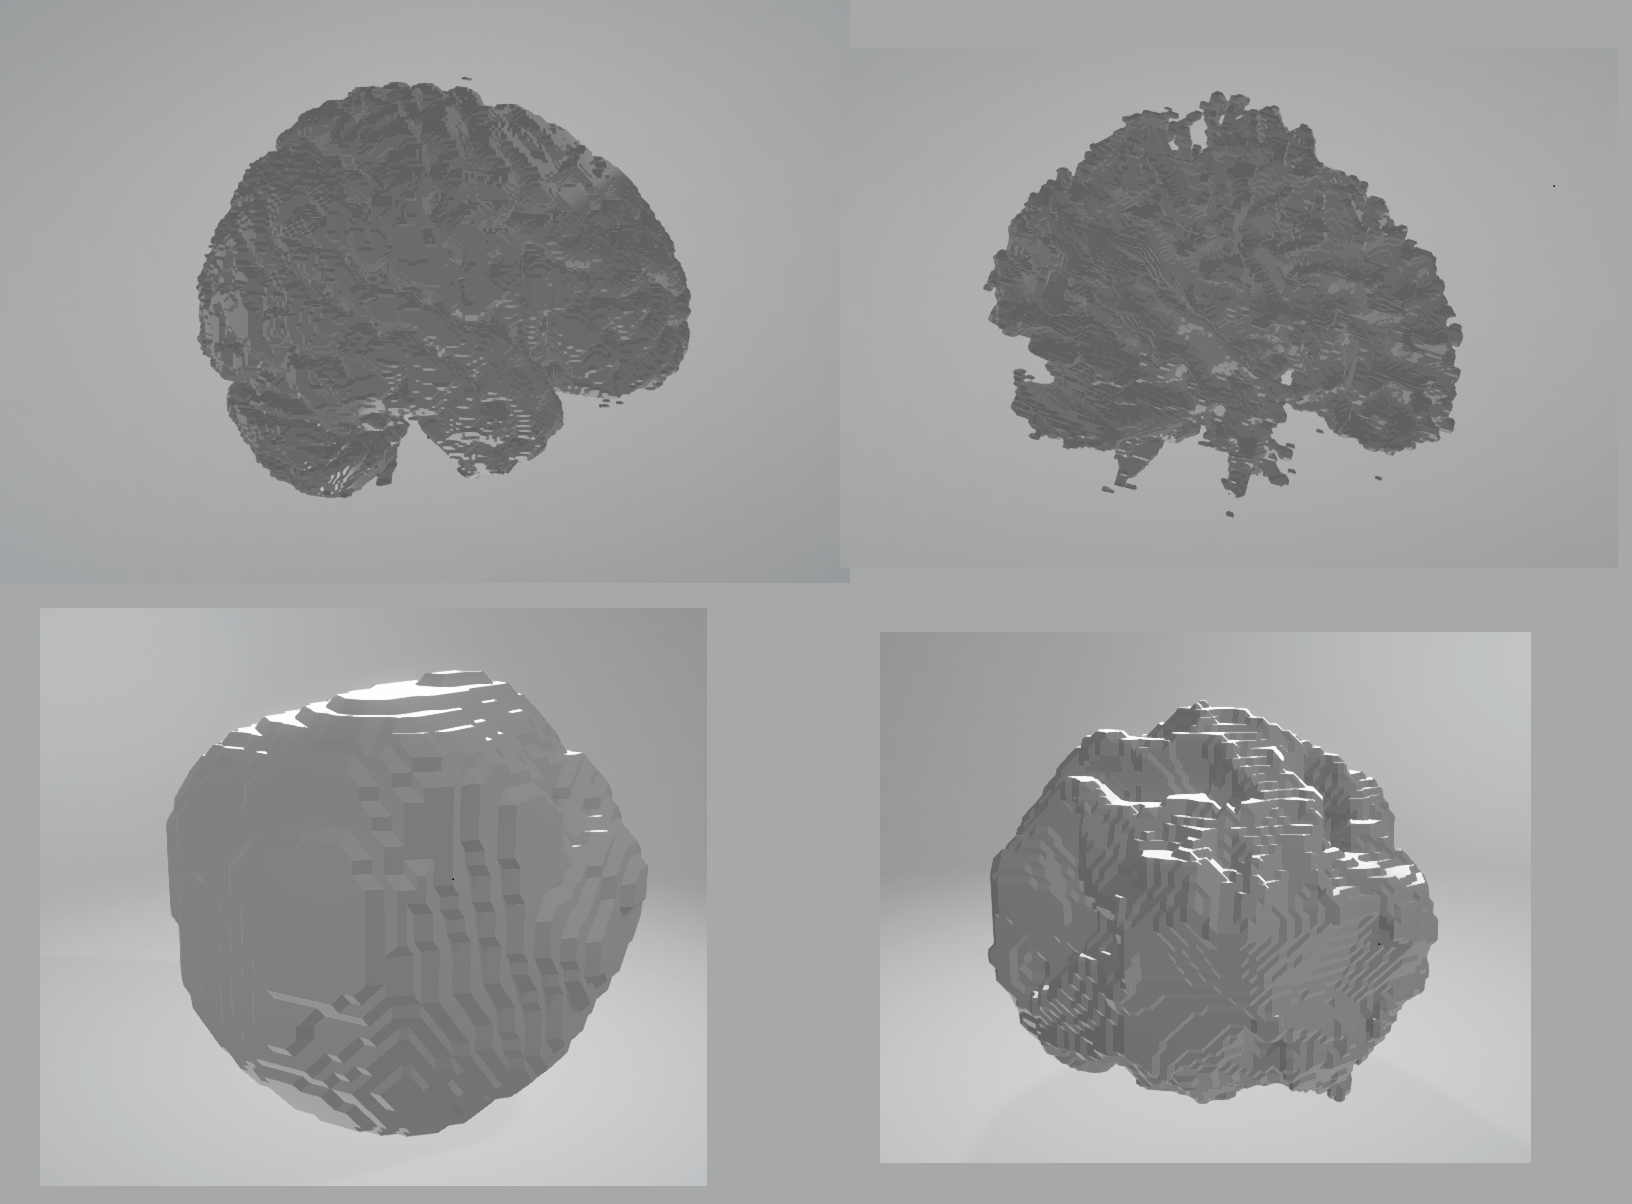
\includegraphics[width=\linewidth]{pictures/resultsMarchingCube.PNG}
  \caption{\textbf{Top Left:} Gray matter \textbf{Top Right:} White matter \textbf{Bottom Left:} Tumor \textbf{Bottom Right:} Abnormal tissue.}
  \label{fig:resultsMarchingCube}
\end{figure}

\begin{figure}[h]
 \centering % avoid the use of \begin{center}...\end{center} and use \centering instead (more compact)
 
\includegraphics[width=\columnwidth]{pictures/general-model.png}
 \caption{Current State}
 \label{fig:general-model}
\end{figure}

\subsubsection{Volume Observations: Opaque and Translucent Views}
The opaque views create a three dimensional form in the viewing space, with defined markings on the brain surface. In figures \ref{fig:noalphared-lateral} through \ref{fig:alphared-front}, our rendering sample depicts an applied red transmission colour.

% \begin{figure}[ht]
%  \centering % avoid the use of \begin{center}...\end{center} and use \centering instead (more compact)
%  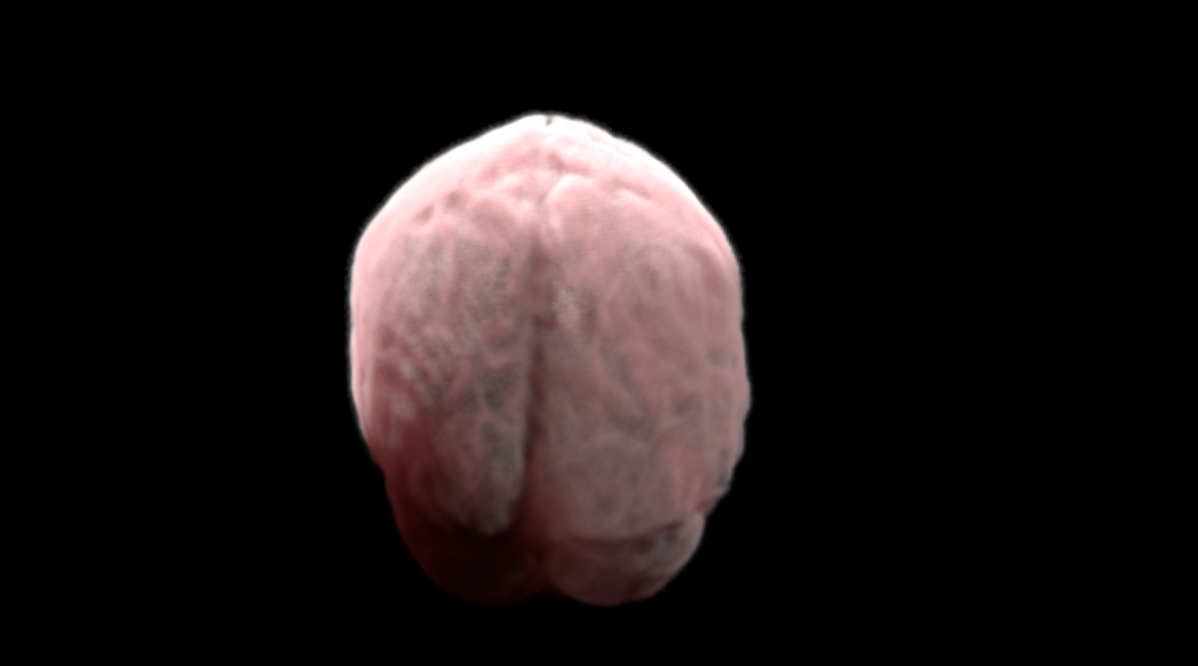
\includegraphics[width=\columnwidth]{pictures/bt-noalphared-front.png}
%  \caption{Opaque MRI Render. Front view.}
%  \label{fig:noalphared-front}
% \end{figure}

\begin{figure}[h]
 \centering % avoid the use of \begin{center}...\end{center} and use \centering instead (more compact)
 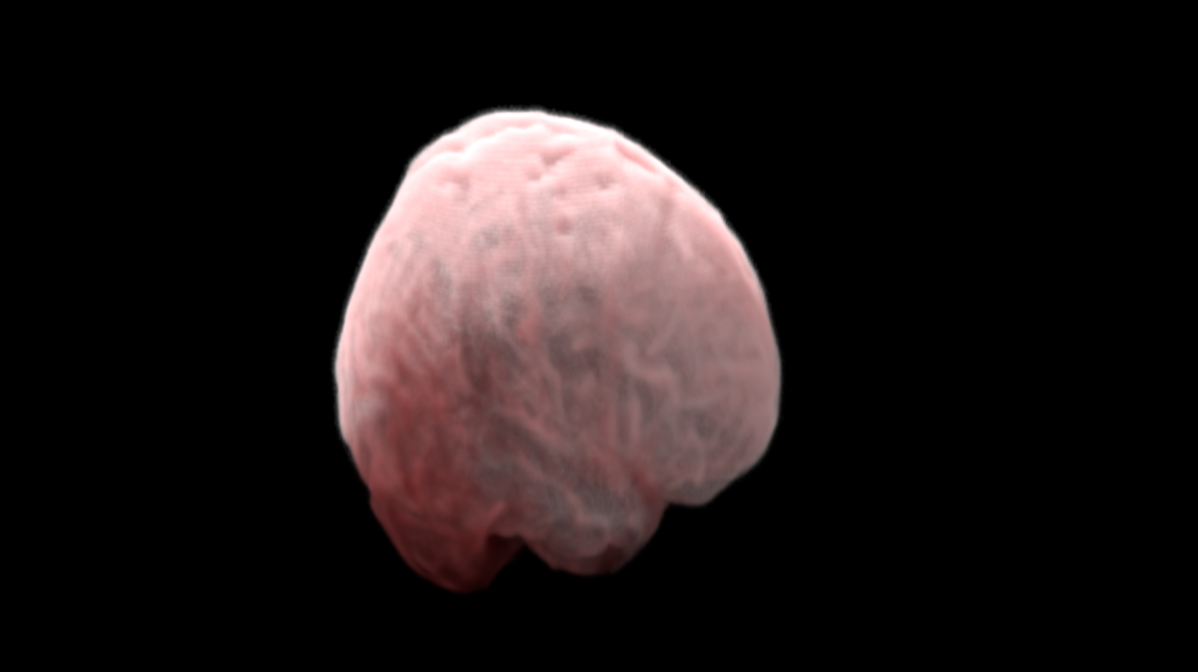
\includegraphics[width=\columnwidth]{pictures/bt-noalphared-lateral.png}
 \caption{Opaque MRI Render. Lateral view.}
 \label{fig:noalphared-lateral}
\end{figure}

\begin{figure}[h]
 \centering % avoid the use of \begin{center}...\end{center} and use \centering instead (more compact)
 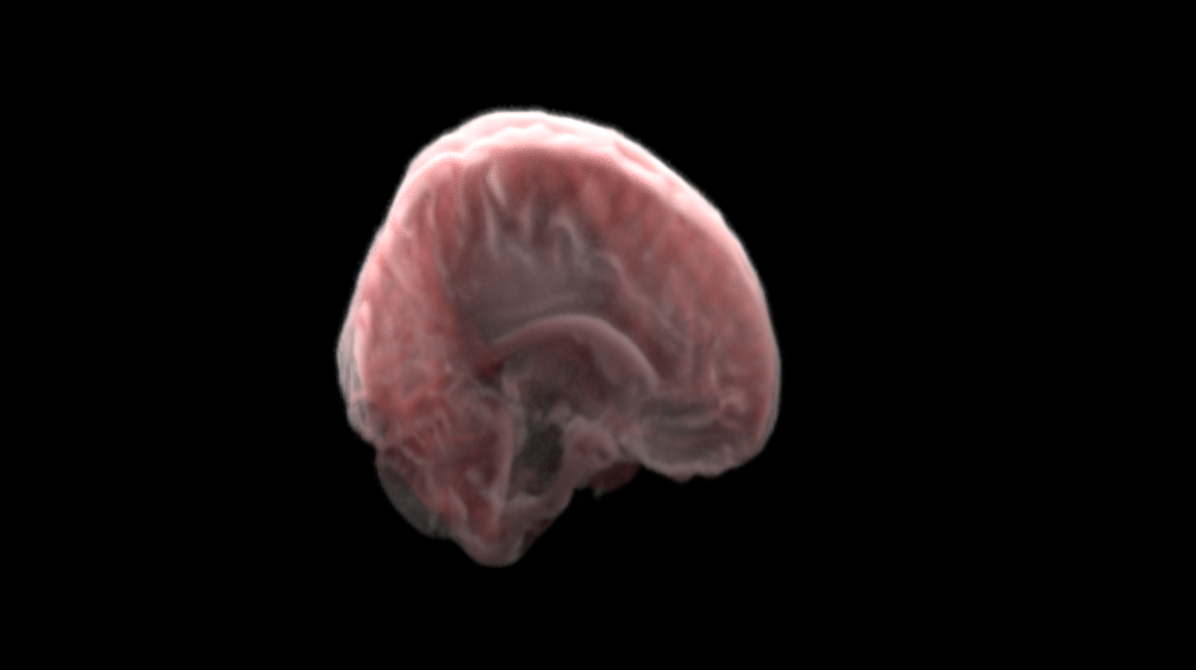
\includegraphics[width=\columnwidth]{pictures/bt-noalphared-lateral-slice.png}
 \caption{Opaque MRI Render. Lateral slice view.}
 \label{fig:noalphared-lateral-slice}
\end{figure}

\begin{figure}[h]
 \centering % avoid the use of \begin{center}...\end{center} and use \centering instead (more compact)
 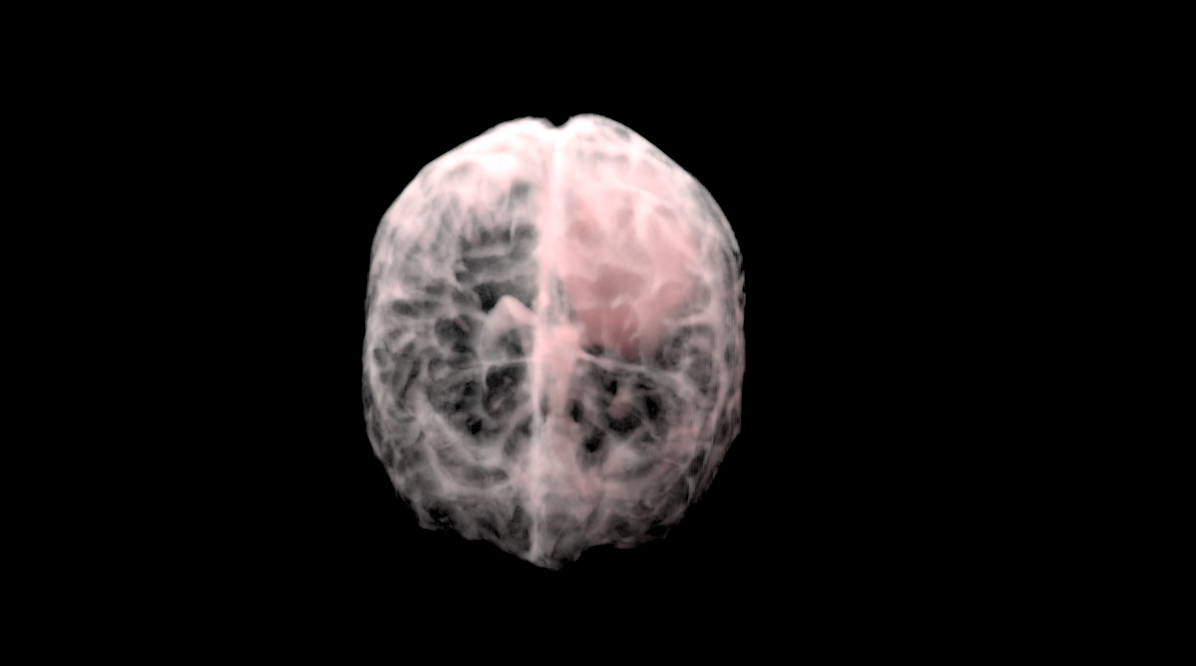
\includegraphics[width=\columnwidth]{pictures/bt-alphared-front.png}
 \caption{Translucent MRI Render. Front view.}
 \label{fig:alphared-front}
\end{figure}

\begin{figure}[h]
 \centering % avoid the use of \begin{center}...\end{center} and use \centering instead (more compact)
 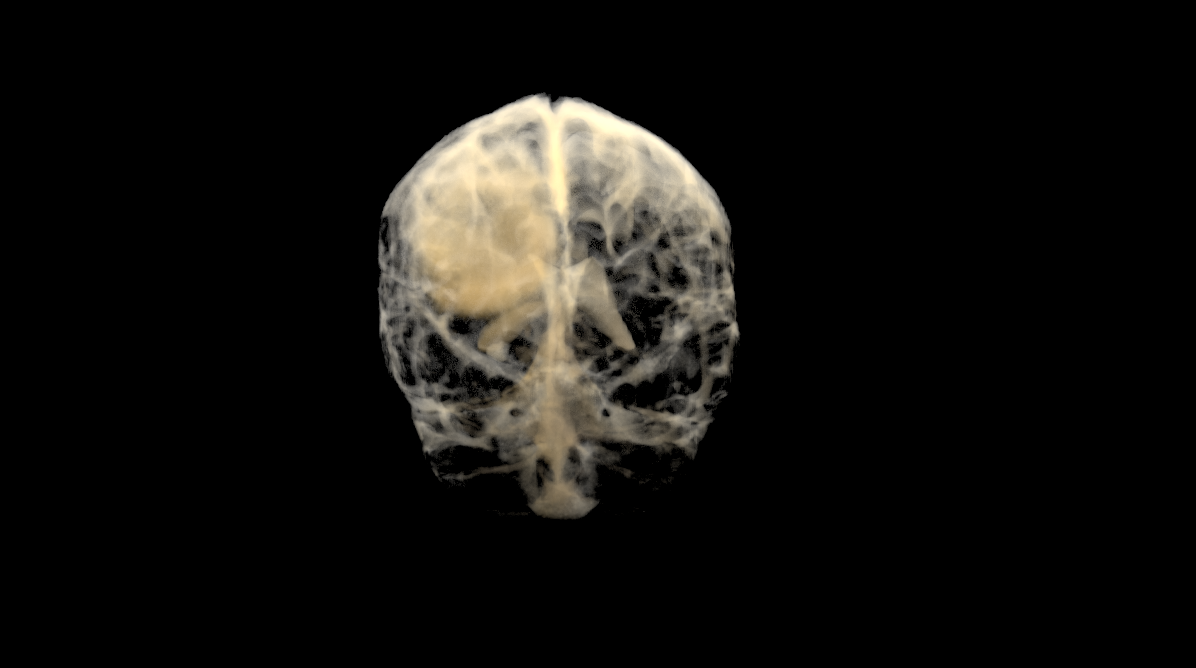
\includegraphics[width=\columnwidth]{pictures/bt-alphalimon-back.png}
 \caption{Translucent MRI Render. Front view.}
 \label{fig:alphared-front}
\end{figure}

Slight opaque regions are revealed from the top down in opaque slices. Translucent slices have a more crystallized look and feel to the image when sliced, however the TC regions are much more prominent.

\subsection{Colour Mapping Methods}
In the CIE 1931 chromaticity diagram, the Y component represents the photopic luminance.  As we know luminance is key to the ability to pinoint detail in segmentation, and the single most important factor in selecting colormaps in this process.  Previous research suggests that luminance is much stronger with colormaps that have two or more interpolation points, and as such has directed our preference towards divergent colormaps and structure colormaps.\\

The search for increased luminance has been the criteria that has steered our research results towards combining forces of an HDR linear workflow, and control of volumetric lighting.  These characteristics of our proposed pipeline are strongly complemented by adding colormaps to the process at either the input stage of MRI data processing or during the volumetric rendering process.  Both methods reveal more insights from the data of the MRI, and create options bringing color snd luminance to the workflows.

\subsection{Pipeline: Proposed Model (Detailed View)}
Our proposal of combined workflows suggests an amalgamation of tasks condensed into three major steps: (1) MRI data preparation, (2) colour mapping, and (3) hologram encoding.  The MRI data preparation involved the extraction of a MRI DICOM or NIFTI medical file of 181 slices for our brain, after which we applied segmentation to isolate the tumour in the image data in traditional DICOM GSDF grayscale.  The colour mapping process was applied to the volume data, and tests show that a divergent and/or structured colormap yield preferred results of highlighting image detail.

\begin{figure}[t]
 \centering % avoid the use of \begin{center}...\end{center} and use \centering instead (more compact)
 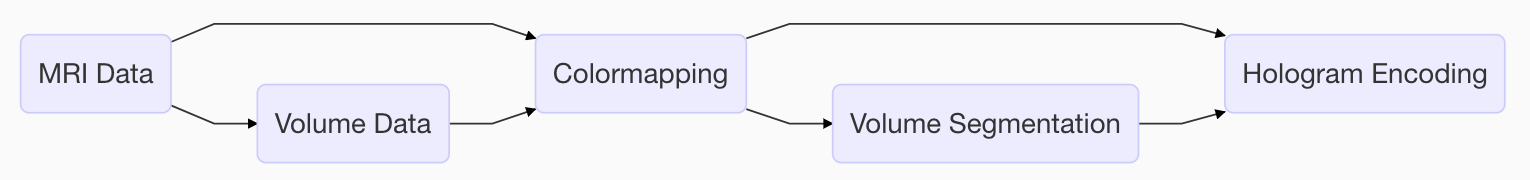
\includegraphics[width=\columnwidth]{pictures/proposed-model.png}
 \caption{Proposed pipeline model}
 \label{fig:proposed-model}
\end{figure}

\subsection{Medical Data Review}
I can't really say anything about this because I do not have any results to speak of.  Meaning we do not have a hologram.  But I was thinking maybe we can create a side by side comparison of the volumetric rendered images with various colour mapping techniques as well as compare them to the geometry based one that was segmented.  Some current ones like gray scale, rainbow and jet, and then we can show our mapping techniques. Then we can talk about the following topics
\begin{itemize}
    \item highlight the advantages of our colour map opposed to others
    \item highlight the importance of geometry vs. volumetric rendering
    \item which one is more true to the medical data (we need Trevor to speak on this)
\end{itemize}








\section{Discussions}
Again we need to see the results to fully talk about this but i was thinking we need to answer the following questions

\begin{itemize}
    \item what are the advantages of our method opposed to others
    \item how did colour play a factor in creating segmentation
    \item how did volumetric rendering play a factor in solving occlusion
    \item in terms of computation how are we better than the current approach 
    \item what are our future work
\end{itemize}


%% if specified like this the section will be committed in review mode
\acknowledgments{}

%\bibliographystyle{abbrv}
\bibliographystyle{abbrv-doi}
%\bibliographystyle{abbrv-doi-narrow}
%\bibliographystyle{abbrv-doi-hyperref}
%\bibliographystyle{abbrv-doi-hyperref-narrow}

\bibliography{template}
\end{document}
